% Selected DSN2027 manuscript; evidence and release provenance are archived separately.
\documentclass[conference,10pt]{IEEEtran}
\usepackage[T1]{fontenc}
\usepackage{cite,amsmath,amssymb,amsthm}
\usepackage{booktabs,array,multirow,graphicx}
\usepackage{url,microtype}
\usepackage[hidelinks]{hyperref}
\newtheorem{definition}{Definition}
\newtheorem{proposition}{Proposition}
% Derived only after all 80 cells of the five-policy native campaign completed;
% roles and SHA in figures/figure_data_v16.json and the campaign FINAL_SUMMARY.
\newcommand{\NativeFullCreditPct}{94.3}
\newcommand{\NativeReadyCreditPct}{42.4}
\newcommand{\NativeSZeroCreditPct}{95.0}
\newcommand{\NativeConsCreditPct}{40.3}
\newcommand{\NativeCreditGainPP}{51.83}
\newcommand{\NativeFullWorkerSeconds}{222.523}
\newcommand{\NativeReadyWorkerSeconds}{326.232}

\begin{document}
\title{RevTrace: Preserving Valid Progress across Trusted Feedback Revisions}
\author{\IEEEauthorblockN{Anonymous submission}\IEEEauthorblockA{Regular paper}}
\maketitle
\begin{abstract}
A stateful inference service can deliver text within its display deadline,
then erase it when a trusted revision confirms the screen. RevTrace
preserves valid progress by coordinating running original
calls, selected results, and whole consumer views, with separate evidence
for eligibility, selection, and support. Every selected transition is
allowed by the original program. In a 24-speaker factorial study the two
retentions remove different withdrawal classes: computation retention
raises avoidable withdrawals from 6 to 17, view retention ends them, and
joint retention leaves neither. On a native recognizer--corrector path
the switches separate again: replacing the view erases all ten supported
views that retained calls meet, keeping it erases none. Retention
delivers \NativeFullCreditPct\% dual-deadline coverage against
\NativeReadyCreditPct\% for completed-result reuse and
\NativeConsCreditPct\% for serial execution, with 31.8\% less worker
time and 23.7\% less energy than reuse; on 15-s natural inputs
certification misses fall from 27 to zero.
\end{abstract}
\begin{IEEEkeywords}
dependable inference, feedback state, incremental computation, speculative execution, streaming ASR
\end{IEEEkeywords}
\section{Introduction}\label{sec:intro}
In an actual streaming-correction run, text appears within its two-second
display deadline, then disappears for 2.176~s even though the selected
update still supports it. Certification also meets its eight-second
deadline (Figure~\ref{fig:continuity_case}(a)). Both deadline tests pass
for this interval, yet the supported result is unavailable during the
gap. Timely first delivery does not establish continued availability.

\begin{figure*}[t]
\centering
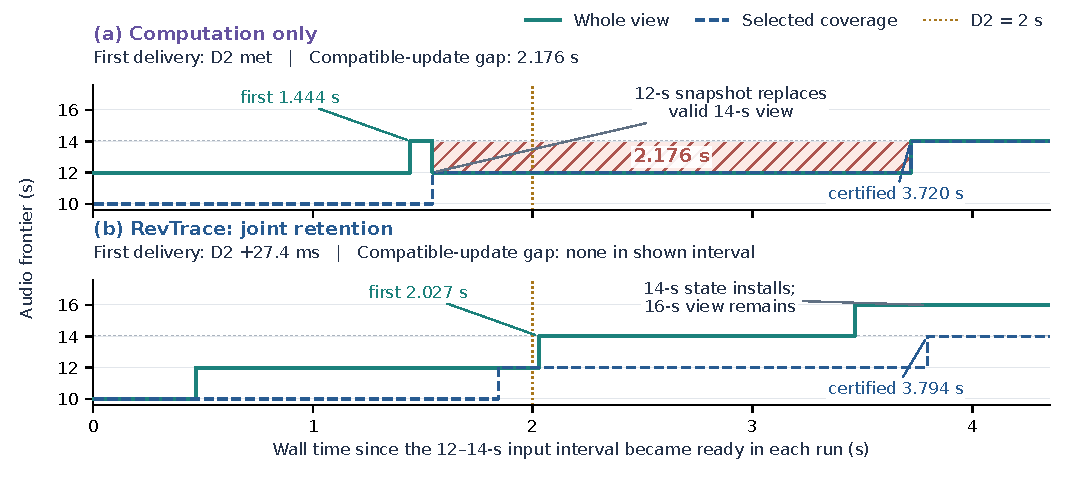
\includegraphics[width=\textwidth]{figures/timely_full_interval_case.pdf}
\caption{Timely delivery can lose supported progress. Two measured
executions of the same complete 12--14-s audio interval in a 16-session
staggered workload, each on its own service clock.
(a) Computation-only delivers 37 code points within D2, then loses the
supported view for 2.176~s before identical text returns.
(b) RevTrace delivers 27.4~ms after D2 and preserves coverage when its
14-s state installs beneath a supported 16-s view; both certified
deliveries meet C8 (8~s).}
\label{fig:continuity_case}
\end{figure*}

We study this problem in inference services whose selected outputs feed
later computation. StreamCorrect, for example, applies a learned
correction to recognition output and feeds the selected correction into
subsequent ASR~\cite{vu2026streamcorrect}. Early execution overlaps these
dependent calls, and early hypotheses can reach a consumer while
selection is still running. A selected correction must then reconcile
computation already in progress, complete results awaiting selection,
and the whole hypothesis currently being read. Preserving useful
progress requires coordinating these objects with the original feedback
program---the complete stateful call that the unmodified recognizer--corrector
pair would issue, as opposed to a stage forecast or a partial result.

The objects need different evidence. A call issued before an update can
have exactly the complete input that the update later selects, while
its own predicted successor is wrong. That call can remain useful, but
only its original correction and update may supply the selected result.
A displayed hypothesis has a separate support path: an update can
invalidate that path while a future call's input is still unresolved.
A worker executes a frozen call, an Owner serializes selected
transitions, and a Consumer maintains the current whole view.
Their decisions must preserve both valid work and the authority of the
original program.

RevTrace coordinates these decisions in one execution protocol
(Figure~\ref{fig:protocol}). It keeps unresolved full calls available
until their own inputs can be resolved, joins complete original results
to the actual selected parent, and preserves the whole visible view
when its support survives application. These are complete-call input
eligibility [EL], original selection authority [AU], and whole-view
support [SUP]. Selected facts become durable before installation; the
Consumer checks their application and reconciles its current view.
Received results remain owned independently of their producer's later
lifetime, and physical ownership is released only after terminal drain.

\begin{figure*}[t]
\centering
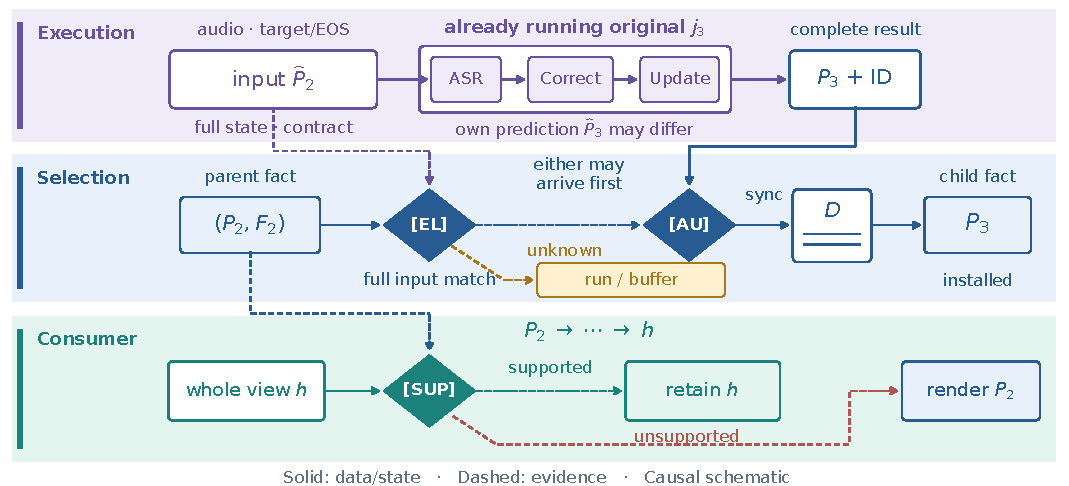
\includegraphics[width=\textwidth]{figures/coordination_protocol.pdf}
\caption{A call, its selected parent, and the Consumer's view use
evidence differently. Call $j_3$ freezes the full conditional input
before the parent's original Correct/Update selects $P_2$; a match
confirms its input while its own prediction may still differ from $P_3$.
Selection joins the complete original result with its actual parent and
owned identity, and the bound fact is synchronized before installation.
The Consumer independently checks the whole view when each fact is
applied. Pending calls may run or buffer without selection. Protocol
schematic, not a measured timing trace.}
\label{fig:protocol}
\end{figure*}

The design builds on dependency tracking, input-bound versions, and
validation before use~\cite{schlangen2011incremental,hammer2014adapton,hammer2015names}.
RevTrace combines them with original neural selection and whole-view
reconciliation so that retained computation becomes supported service.
A version bound to the complete call input supplies the same eligibility
witness: our version-DAG control shares the core input, retention,
selection, and support conditions, and its matching native handovers
show that the coordination admits multiple implementations.

The joint objective has a measurable consequence. In the prespecified
24-speaker Qwen setting with 2-s feedback and staggered arrivals,
computation retention raises total withdrawals from 12 to 17, including
avoidable withdrawals from 6 to 17, while ending the withdrawals that
later feedback itself forces. Retaining valid computation alone
nearly triples avoidable withdrawals for a simple reason: without
retention a speculative branch advances at most one step past the
certified frontier, whereas with it the branch runs several windows
ahead, so installing a compatible 12-s snapshot beneath a displayed
14-s view erases supported text unless the Consumer reconciles that
view (Figure~\ref{fig:continuity_case}(a)). View retention alone
eliminates avoidable withdrawals but delivers 628.435~s of
audio within both deadlines; joint retention delivers 680.760~s with
zero withdrawals. Preserving computation does not by itself preserve
the compatible view, and preserving the view does not recover discarded
computation.

A separate native comparison repeats both switches under the original
recognizer--corrector task, with a policy that issues nothing before
confirmation. All policies use the same two complete FP32 workers,
selection and view-support checks, and dispatcher. Across eight speakers,
in-flight retention delivers \NativeFullCreditPct\% dual-deadline
coverage against \NativeReadyCreditPct\% for completed-result reuse and
\NativeConsCreditPct\% for serial execution. Replacing the view instead
of keeping it clears all ten supported views that retained calls meet,
and buys 1.000~audio-s; keeping it erases none. Retention reduces
worker occupation by 31.8\% and two-board energy by 23.7\% against reuse;
against serial execution it spends 12.6\% more worker time for 7.4\%
less energy, serving the stream earlier rather than doing less work.

We make three contributions:
\begin{itemize}
\item \textbf{A dependability problem and service contract.} We identify
  avoidable withdrawal of supported progress after timely first
  delivery, and define the call, selected-result, and whole-view
  objects needed to distinguish continued availability from first
  arrival (Sections~\ref{sec:contract}--\ref{sec:continuation}).
\item \textbf{An executable joint protocol.} Complete-input witnesses,
  durable original selection, independent Consumer reconciliation,
  and physical ownership rules coordinate retention. Each session's
  selected facts form an execution allowed by the original program;
  replay adds no original transition. A selected-trace argument and
  executable checks establish these properties
  (Sections~\ref{sec:continuation}--\ref{sec:protocol}).
\item \textbf{Mechanism and end-to-end evidence.} Factorial controls
  expose the interaction between work retention and visible
  continuity. Native full-program comparisons measure the
  recomputation avoided by in-flight retention, with complete resource
  accounting, process-failure checks, and same-resource multi-session
  controls (Section~\ref{sec:eval}).
\end{itemize}

\section{System and Feedback Contract}\label{sec:contract}
\subsection{The original feedback program}
A session consumes immutable audio released over time. Its original
program recognizes candidates, selects a correction, and updates the
state used by the next call. In StreamCorrect, selected corrections feed
later ASR~\cite{vu2026streamcorrect}. RevTrace changes when calls run and
which progress remains visible while preserving this original program.
Write $s\mathrel{\Rightarrow_{\mathcal A,X}}t$ for a transition allowed
by the original program $\mathcal A$ on accepted immutable input $X$;
this relation may be nondeterministic.

The adapter declares a closed cut $x=(F,P)$, where $F$ is the input
frontier and $P$ contains all mutable cross-call state that can affect
subsequent inference or selection. The execution contract binds the
model, audio identity, decoding, state encoding, and output-to-text
transformation. A selected fact is
\begin{equation}
 C=(v,F,Z_C,P_C,T_C),
 \label{eq:canonical}
\end{equation}
where $v$ identifies the selected version, $Z_C$ is the complete original
result, and $T_C$ is its bound text. Selection is distinct from human
transcription accuracy. The adapter also records processing coverage:
an original buffer-only transition need not earn new neural-processing
credit, and advancing a state frontier need not add characters.

A job freezes its complete input before dispatch. A recorded node has
\begin{equation}
 q_j=(a_j,P_j^-,b_j,\chi_j),\qquad
 n_j=(q_j,\tau_j,Z_j,P_j^+,T_j),
 \label{eq:node}
\end{equation}
with start cut $(a_j,P_j^-)$, target $b_j>a_j$, and $\chi_j$ binding the
remaining inputs: accepted audio, EOS, configuration, and original job
identity. The node type $\tau_j$ distinguishes a stage forecast from a
complete original call. A forecast may become available while original
correction is still running; completion requires the original selection
and update, including their declared buffer-only path. The frontier
records input progress rather than a word-to-audio alignment.

State equality means equality of the complete declared encoding under
the same contract. The native adapter carries audio buffers, token
groups, context, alignment position, and decoder configuration at a
clean-cache boundary. The core Qwen adapter carries feedback prompt
tokens without cross-call numerical KV caches. Text alone cannot witness
equality of an omitted cursor, token state, or numerical cache. Telemetry
and resource accounting are recorded separately.

\subsection{Selected facts, calls, and the actual view}
An \emph{Owner} serializes selected transitions for each session. The
native runtime has two protected workers, each hosting the complete
original recognizer--corrector--update pipeline. Either can run from a
selected cut or a conditional forecast. A Supervisor preserves accepted
input obligations and monitors processes; an actual FIFO Consumer applies
the Owner's publications. Durable storage records the selected prefix.
The earlier factorial runtime uses the same logical roles with separate
provisional and protected-selection paths.

The Consumer's whole view $h$ binds text and a visible frontier to a
complete published path from its selected root to its displayed tip.
It may be ahead of the selected state. A path node is not selected merely
because its text was displayed. Conversely, an already received complete
result may remain usable after its producer exits. Call eligibility,
selection of an original result, support of $h$, and physical resource
ownership therefore refer to different objects.

Every accepted input remains an obligation until original certified
processing covers it. Rejecting a branch, cancelling a call, or replaying
an old fact neither removes that obligation nor resets its arrival
clock. Exact mode never trades this rule for a deadline: lateness cannot
authorize an uncertified selected transition.

\subsection{System and failure model}\label{subsec:failure_model}
The argument assumes one legitimate serial writer, faithful execution of
frozen inputs and original selection code, sufficient declared state,
unambiguous encoding, collision-resistant digests, and storage honoring
successful synchronization. Workers and host components faithfully
execute the original program; its allowed relation accommodates
nondeterministic execution.

The native failure model covers worker or Owner-group crash-stop,
late/duplicate messages, and fenced physical incarnations on an intact
filesystem. Supervisor, ingress ledger, actual Consumer, power observer,
and recoverable storage survive. Controlled wrong-input injections in
Section~\ref{sec:eval} exercise the input and identity rejection guards.

\section{Coordinating Calls and Whole Views}\label{sec:continuation}
\subsection{One original call through a revision}
RevTrace coordinates an original call that starts before its input is
selected, its eventual use at the actual parent, and the whole view that
the Consumer currently reads. Figure~\ref{fig:protocol} follows call
$j_3$ on forecast $\widehat P_2$. Selecting a matching $P_2$ can preserve
that call; it does not endorse $j_3$'s own forecast $\widehat P_3$.
Original Correct/Update must still produce its complete result $P_3$.
Independently, the Consumer checks whether its current view is supported
when $P_2$ is applied. Keeping computation alone does not keep that view.
Table~\ref{tab:decision_objects} maps each use to its governing judgment.


\begin{table}[t]
\centering
\caption{Evidence and permitted actions for calls, results, and views.}
\label{tab:decision_objects}
\begingroup\small\setlength{\tabcolsep}{3pt}
\begin{tabular}{@{}>{\raggedright\arraybackslash}p{.27\columnwidth}>{\raggedright\arraybackslash}p{.35\columnwidth}>{\raggedright\arraybackslash}p{.33\columnwidth}@{}}
\toprule
Object & Judgment & Permitted use\\
\midrule
{[EL]} Frozen call input & Confirmed, pending, or refuted by actual full-state evidence & Continue confirmed or pending work; not select its prediction.\\
{[AU]} Original full result & Owned result on the actual current parent & Append a selected fact, then install after synchronization.\\
{[SUP]} Current whole view & Complete support under this actual application & Preserve the ahead view; not certify its forecast.\\
\bottomrule
\end{tabular}\endgroup
\end{table}

\subsection{Retain the call without selecting its prediction}
\label{subsec:native_full_calls}
In the native pipeline, ASR produces ordered beam candidates and the
open state needed by original correction. Before learned correction
finishes, the same update tail with a typed first-beam identity prediction
can expose provisional closed state $\widehat P^+$. This is a forecast,
not evidence that original Correct/Update selected it. The other worker
may execute the next \emph{complete original call} on that conditional
input. Both workers still execute ASR, original correction, and update.

For that call, [EL] compares its immutable start with actual selected
state at the same frontier. Equality confirms the input; disagreement
refutes it; without such a witness it is pending. Pending is not false.
A running call can continue, or its full result can wait in a ready bank,
without obtaining selection authority. A known same-frontier mismatch,
an already covered target, or a lifecycle fence can justify rejecting
use. An earlier ancestor mismatch alone does not refute an unresolved
future complete input. Conservative policy fences may discard work,
but are distinct from a proof that its input is wrong.

The witness can have different representations. The core runtime checks
a matching complete boundary and the unbroken recorded suffix to the
actual tip. The native full-call runtime checks the call's own complete
start. A version uniquely bound to that input can carry the same
evidence; a coarse birth version need not. Safe unconditional in-flight
retention can also let work finish and validate it before use. These
representations can share a complete-input witness, while [AU] still
governs selection and [SUP] governs the actual whole view.

In the factorial study, $R$ enables computation retention under its
declared witness, and $S$ enables retention of a supported ahead view.
Disabling either retention action preserves the shared safe-use checks.
The native policy comparisons likewise retain original selection and
whole-view validation while varying dispatch, in-flight retention,
ready-result retention, or cooperative early stopping.

\subsection{Selection is a serialized join}
The selected parent can change after dispatch. The Owner therefore joins
the worker's completed result with the parent that is current at
selection. It first binds that result to the registered call's original
identity, frozen start and target, contract, and original selection/update
record. It selects the result only when its full start equals the
installed parent. A future result waits; completion order cannot create
a missing parent, and refuted or covered work cannot supply a new fact.
Table~\ref{tab:coordinator} gives the transaction.

\begin{table}[t]
\centering
\caption{The selection transaction, followed by independent reading and
physical retirement.}
\label{tab:coordinator}
\begingroup\small\setlength{\tabcolsep}{3pt}
\begin{tabular}{@{}p{.10\columnwidth}>{\raggedright\arraybackslash}p{.84\columnwidth}@{}}
\toprule
Step & Coordinator action\\
\midrule
1 & Bind the full result to its unchanged owned call; buffer while its complete input is pending.\\
2 & Under serial selection, revalidate that input against the installed parent and the durable writer's root for this session.\\
3 & Append the original result, parent, and identity; flush and synchronize the bound record. An uncertain outcome freezes new writes.\\
4 & Recheck the parent after the callback, install only with the bound durable receipt, and publish this installation's own view snapshot.\\
Read & The Consumer validates fact order and its actual parent, then separately reconciles its whole view.\\
Retire & Reuse a physical slot only after its matching terminal/drained outcome or confirmed process and CUDA release.\\
\bottomrule
\end{tabular}\endgroup
\end{table}

\paragraph{The invariant established by these actions}
For one session, let $D=(d_1,\ldots,d_n)$ be its ordered facts within the
verified journal prefix, with genesis $x_0$ and successive endpoints
$x_1,\ldots,x_n$. Other sessions may interleave in the journal. The invariant
has three parts: each new $d_i$ binds a distinct owned original call
from $x_{i-1}$ to its original complete result $x_i$; the Owner's
installed cut is some verified prefix position $x_k$, $0\leq k\leq n$;
and the Consumer applies only ordered facts from this prefix, while
provisional views remain a separate lane. In particular, successful
synchronization followed by a crash before installation permits
$k=n-1$. Installed state is a durable \emph{prefix}, not always its tail.

\begin{proposition}[Selected-trace refinement]
\label{prop:refinement}
Under the contract and failure assumptions of
Section~\ref{sec:contract}, the coordinator's guarded actions preserve
this invariant. Projecting onto distinct new selected facts yields an
execution allowed by the original program $\mathcal A$. Replaying an
existing fact adds no original transition.
\end{proposition}
\begin{proof}
Genesis supplies the initial prefix. Dispatch, forecasts, completion,
waiting, and rejection do not extend $D$. For an append, call binding
and faithful execution supply an original result
$s\mathrel{\Rightarrow_{\mathcal A,X}}t$ on its frozen input. The serial
pre-append checks compare $s$ with both the installed parent and the
writer's verified per-session tail. Hence $s=x_n$; the new record extends
the old allowed prefix by that original edge. Identity consumption and
duplicate rejection prevent another new edge from the same owned outcome.
Synchronization precedes installation; installation only advances $k$.
If the callback is uncertain, writes freeze rather than grant a new
installation. Recovery validates the complete recorded prefix and
replays those identities; it executes no new neural transition.
The Consumer's sequence and parent checks preserve its prefix.
Induction establishes the claim. The omitted protocol actions are
stuttering in this selected-fact projection~\cite{schneider1990statemachine,abadi1991refinement}.
\end{proof}

Proposition~\ref{prop:refinement} needs less than bit-exact repetition.
Its premise is that the appended edge is the one the original program
produced on its frozen input, not that two independent executions agree
bit for bit, which the contract's nondeterministic relation $\mathcal A$
already permits. The runtime supplies that premise operationally: a
channel bound to the physical worker incarnation returns each result
under the identity of the call that produced it, and all 32 native runs
match an independently generated reference.

The result retains its original identity through this join. A complete
result already received and owned before a worker-only fence can remain
usable with its original incarnation. Owner-group recovery instead
replays durable facts, and leaves uncommitted old-Owner work outside the
new write namespace. Section~\ref{sec:protocol} describes the corresponding
physical ownership rules.

\subsection{The Consumer checks its whole view}
A call input and a displayed path can diverge. For a recorded node,
the provisional dependency relation is
\begin{equation}
 (F,P_C)\xrightarrow{n_j}(b_j,P_j^+)
 \quad\text{when}\quad a_j=F\ \land\ P_j^-=P_C,
 \label{eq:edge}
\end{equation}
under the same full-input and identity contract. Write $C\leadsto h$
when complete published nodes form an unbroken path from $C$ to the
actual displayed tip. This relation checks support of a forecast or
full node; it does not turn a forecast edge into an original selected
transition.

At an actual canonical application, [SUP] checks the Consumer's current
whole view, not merely a convenient Owner node. A matching complete
boundary permits removal of the covered path prefix while retaining its
entire supported suffix. Missing, ambiguous, or mismatching ancestry
cannot justify retention. The bound text, frontier, original results,
and current root are checked together; there is no uncertified suffix
splice or caller-supplied compatibility flag.

\begin{proposition}[Continuity at a compatible application]
\label{prop:continuity}
Immediately before an authorized canonical application at frontier $F$,
let the actual whole view $h$ be ahead of $F$. If the incoming selected
fact $C$ satisfies $C\leadsto h$ and no independent withdrawal mode is
invoked, that application advances the selected lane and preserves $h$
unchanged.
\end{proposition}
\begin{proof}
The Consumer first validates publication authority, order, and the
durable parent. At the matching boundary, reconciliation removes only
the covered path prefix. The remaining suffix has the same original tip,
text, and frontier as $h$. Old or duplicate publications are rejected
before changing these lanes. Thus this application does not withdraw
$h$.
\end{proof}

An incompatible application may require withdrawal, and later original
results may revise text. This property protects the supported whole view
at each compatible application.

\subsection{A call can outlive an ancestor prediction}\label{subsec:ancestor_outlives}
Consider an allowed state-convergence case, with all referenced audio
already accepted and its boundaries numbered 0--3. Call $A$ runs from $x_0$ and forecasts
$\widehat x_1$. Call $B$ starts there and completes $x_2$ before $A$;
its future result waits, freeing a worker. Call $C$ can now start from
$x_2$ while its birth root is still $x_0$. Suppose $A$ then selects
$x_1\ne\widehat x_1$. This refutes $B$'s input, but says nothing yet
about $C$'s complete input at frontier 2. If an original recomputation
$D$ from $x_1$ produces $x_2$, $C$ becomes confirmed and may supply its
own complete result $x_3$. The selected execution is
\begin{equation}
 x_0\xrightarrow{A}x_1\xrightarrow{D}x_2\xrightarrow{C}x_3.
\end{equation}
It is contiguous: no skipped frontier or rollback is needed. $B$'s
output equality with $x_2$ never authorizes $B$, whose input was wrong.
$C$ retains its identity and still executes original Correct/Update.
If the Consumer had displayed the old path through $\widehat x_1$,
that path would separately fail [SUP].

An executable three-frontier, four-call control constructs this case.
It separates a call's own complete input from its ancestral provenance:
$C$ can become usable even after its tracked ancestry fails. A strict
ancestor-revocation policy may safely discard $C$, but then forgoes this
reuse. A policy that preserves the opportunity needs a witness for $C$'s
actual input; input-bound versions can supply it. Matching expected-parent
handovers likewise support multi-step compatible chains. This finite
protocol case establishes the opportunity rather than its prevalence
in the native traces.

\subsection{Executable checks and implementation correspondence}
\label{subsec:native_refinement}
A separately frozen, hand-written Python state machine checks the
invariants over explicit protocol actions. Two symbolic values represent
equality or disagreement of complete opaque state; original C/U is an
allowed, potentially nondeterministic relation. A custom breadth-first
search checks 6,231 states/11,142 edges with two frontiers, at most three
issued jobs and no fault; and 14,074 states/25,799 edges with one frontier,
at most two issued jobs and at most one fault. Both explore to depth 12, leaving
2,144 and 2,828 depth-boundary states unexpanded. The 35 named controls
comprise the original 27 legal/mutation cases and eight phase/action
checks. They verify that Sync extends the fact prefix while Install and
Replay use existing facts. Constructed mutations expose using a forecast
as C/U, withdrawing a compatible view, and attaching a later root to an
earlier publication. These are checks of a bounded protocol model.

Source-level protocol controls and an independent trace checker connect
actual dispatches, full-call receipts, durable facts, publications, and
Consumer applications to the same obligations. The selected-fact
projection connects durable append, installation, and replay to the
original transition relation. Separate application checks evaluate the
actual Consumer's retained read view. The model explores protocol
interleavings; the trace checker binds those obligations to recorded
runtime actions.

\section{Implementation and Reliable Execution}\label{sec:protocol}
\subsection{Executing an original call}
A dispatch freezes the complete model input, source audio range, target
frontier and execution contract. Each native FP32 worker executes the
original inference, selection and feedback-update code. Its early ASR
observation can supply a typed provisional view while original correction
continues; its complete result follows the original C/U path.

All native policies use the same work-conserving dispatcher. It first
considers eligible calls from actual selected inputs across sessions,
then conditional calls, and rotates among eligible sessions. It registers
and sends one dispatch before reconsidering the next free slot.
Conservative can therefore use both GPUs for distinct sessions under the
same resource budget. The policy differences concern which outstanding
calls survive revisions, as evaluated in
Section~\ref{sec:eval}.

\subsection{Logical invalidation and physical ownership}
Dispatch and receipt identities bind the session, Owner namespace,
monotonic job number and physical worker incarnation, following established
RPC identity principles~\cite{birrell1984rpc}. Exact duplicates and fenced
messages are rejected locally. They neither modify selected state nor
release a newer job's slot. Contradictory contents from a currently owned
call freeze further writes.

A retention decision does not terminate GPU execution. In the native
runtime, a known-input mismatch or covered target can request a cooperative
exit at the checkpoint before learned correction. A worker either returns
a complete original result or acknowledges cancellation without a partial
feedback state. Cleanup and device synchronization precede its terminal
receipt. If completion wins the race, the returned result still passes
the original input and selection checks. UIR suppresses these early-exit
requests while keeping the same end-use checks.

Per-incarnation channels bind the message stream to its physical producer.
After an unexpected channel close, complete received frames are validated
before the channel is sealed. Replacement requires confirmed process
exit, released CUDA ownership and joined receivers. In the batched core
instance, a completed row can be used before other rows finish, but the
batch lease ends only after every terminal row and device synchronization.
Neither a logical fence nor a masked row is charged as freed computation.

\subsection{Durable selection and recovery}
An exclusive writer records the full parent and next states, original
correction and returned IDs, owned job and relevant epochs. Framing,
checksums and chaining bind the record; synchronization precedes
installation and publication, following conventional write-ahead
rules~\cite{mohan1992aries}. A successful callback returns the receipt for
that record. An uncertain append or installation outcome freezes writes
until recovery establishes the verified prefix.

\label{subsec:native_resilience}
For an Owner-group failure, the Supervisor confirms the end of old
physical ownership, advances the Owner namespace, and replays the verified
durable prefix to the surviving Consumer before starting the replacement
Owner. Only an incomplete final frame may be discarded; complete
corruption fails verification. Replay preserves the original fact and
job identities. Workers cold-start and continue from the recovered
selected input, using the original ingress clocks.

The sync--install distinction has an observed counterpart. In two repeats
of an earlier Fullcall fault case, journal sequence 5 was synchronized when
the original Owner was terminated before installation. During recovery
to the next Owner epoch, the surviving Consumer replayed that same fact
with its original job identity. For these two facts, the counts of
durable records, original-Owner installations, and Consumer uses were
$2/0/2$. This instantiates the sync--install gap permitted by
Proposition~\ref{prop:refinement}: replay used the existing edge without
adding a neural transition.

Twenty-four further fault cells on one development source exercise six
conditions under both policies. No cell installs illegally or accepts a
rejected mutation. Recovery cost splits by what must be rebuilt: worker
faults resume in 1.8--2.3~s against a surviving model, while Owner-group
faults pay 64.6--108.1~s to rebuild the worker group. No fault cell meets
its deadlines, so these trials establish the absence of an illegal
transition and a bound on recovery rather than continued timeliness. One
condition prices retention directly: when the Owner dies after the
durable install, retaining needs 101.8--104.4~s and 26.5--27.2~kJ against
83.9--87.1~s and 22.4--24.2~kJ, because more outstanding work survives to
be re-driven. Retention moves cost onto the recovery path instead of
paying it in steady state.

An independent audit of that earlier runtime also bound 3,976 selected
and 9,068 provisional applications across 36 traces, and verified
preservation at all 90 compatible-ahead applications.

\phantomsection\label{prop:continued_service}
After finitely many supported failures, eventual progress requires readable
storage, terminating original calls, eventual worker release and loading,
and fair Owner/Consumer scheduling. Loading and replay remain part of
post-fault service time; destroying a model process incurs its actual
reconstruction cost even when an acquired result survives.

\subsection{Keeping control history bounded}
Active calls, ready results, delivered views and unacknowledged
publications pin their required evidence. Acknowledgment releases
publication references, not arbitrary computation dependencies. Monotonic
issue high watermarks prevent old identities from being reissued after
collection. Unreferenced terminal and diagnostic windows are bounded and
streamed to disk. These are bounds on control history; audio, cumulative
text and model state retain their separately measured costs.

\section{Evaluation}\label{sec:eval}
\subsection{Questions, comparisons, and service accounting}
We evaluate how retained computation becomes continuously available
service, when an in-flight original call can be used, and how publication
and resource choices affect those benefits. The factorial study tests
joint computation/view retention; the native study repeats both switches
under the original recognizer--corrector task, with a no-speculation
anchor. Both record
actual Consumer applications and preserve every offered input obligation.

The core study uses Qwen3-ASR~1.7B~\cite{shi2026qwen3asr} on two 24-GB
RTX~3090s. Private and Authority workers use FP16 and FP32; batch delivery,
selection, validation, and persistence are shared. Twenty-four
metadata-selected LibriSpeech speakers~\cite{panayotov2015librispeech}
form three disjoint eight-speaker cohorts. The primary Qwen setting
offers 714.110~audio-s per arm, with 2-s feedback and arrivals staggered
by 0.25~s. Physical early exit is disabled.

Native execution uses two complete FP32 workers on the same two GPUs,
the original StreamCorrect ASR, correction, and update path
~\cite{vu2026streamcorrect}, and 500-ms inputs without VAD. The main
comparison crosses five policies with eight prespecified AISHELL-1
speakers~\cite{bu2017aishell}, one complete 8.138--9.000-s utterance each,
and two fresh repeats per policy; repeats stay within speaker pairs.

For offered interval $i$, duration $w_i$, ready time $r_i$, first actual
visible coverage $d_i$, and first original certified coverage $c_i$, we
report
\begin{equation}
 A_{2,8}=\sum_i w_i\,\mathbf{1}
 \{d_i-r_i\leq2\ \land\ c_i-r_i\leq8\}.
 \label{eq:credit}
\end{equation}
Every offered interval, including partial EOS tails and missing
observations, stays in the denominator. Whole-run passes require
offered-frontier display P99$\leq2$~s and certification P99$\leq8$~s.
Continued availability is measured separately from first delivery: a
withdrawal removes audio-seconds from an already-displayed view, and
the \emph{gap} integrates those removed audio-seconds over the wall
time they stay unavailable, so it is zero only when no displayed
coverage is erased.
Worker occupation sums elapsed worker-job intervals; both-board energy
runs from service origin through confirmed physical model drain.
Loading/warmup precedes normal service, while replacement and outstanding
work retain the original clocks. Reference generation is accounted
separately.

\subsection{Does retained computation remain available to the Consumer?}
We cross computation retention $R$ and supported-view retention $S$,
keeping selection authority and application safety checks common.
Table~\ref{tab:factorial_tradeoff} puts timely credit, withdrawal, and
gap in the same comparison. Relative to snapshot/recompute, computation-only
adds 1.41 percentage points of coverage but raises total withdrawals
from 12 to 17 (avoidable: 6 to 17). View-only reduces total withdrawals
to one and avoidable withdrawals to zero, while coverage falls by
3.60 points. Among these four arms, joint retention improves coverage
by 3.73 points and eliminates withdrawals
(Fig.~\ref{fig:main_evidence}).

\begin{table}[t]
\centering
\caption{Primary staggered factorial comparison: 714.110 offered
audio-s and 368 offered frontiers per arm. Withdrawals are classified
at the actual Consumer; the count in parentheses is the avoidable
subset. Gap is the time integral of removed, not yet restored
displayed audio.}
\label{tab:factorial_tradeoff}
\begingroup\small\setlength{\tabcolsep}{2.5pt}
\begin{tabular}{@{}lrrr@{}}
\toprule
Arm & $A_{2,8}$ (s) & Withdrawals & Gap (audio-s$\cdot$s)\\
\midrule
$R_0S_0$ Snapshot & 654.115 & 12 (6) & 15.458\\
$R_0S_1$ View only & 628.435 & 1 (0) & 0.258\\
$R_1S_0$ Compute only & 664.150 & 17 (17) & 30.258\\
$R_1S_1$ Joint & 680.760 & 0 (0) & 0.000\\
\bottomrule
\end{tabular}\endgroup
\end{table}

Withdrawals separate into two classes, and one class follows each
factor. A withdrawal is avoidable when the cleared view is compatible
with the projection that installs, and necessary when later feedback
contradicts that view. Necessary withdrawals are absent in both arms
that retain computation and present in both that do not (six and one);
avoidable withdrawals are absent in both arms that retain the view and
present in both that do not (six and seventeen). Only the joint arm is
empty in both, so coordination is not two gains added: it is the
intersection of two failure modes with different causes. The reason is
content rather than timing: an ahead view built by a complete call on a
frozen input can be overtaken in time but not contradicted in content,
whereas whether a compatible view survives application is a publication
decision.

Neither the count nor the credit fixes how long a reader loses text.
Under the snapshot baseline 12 withdrawals fall on the 368 offered
frontiers, 3.3 per 100, in all three cohorts; they remove 10.5~s of
already-displayed audio and keep it unavailable for
15.5 audio-s$\cdot$s. Computation retention raises the three
quantities to 17, 18.6~s, and 30.3. The gap sums both classes, which
is why view-only still shows 0.26: that residue is its single necessary
withdrawal, where later feedback contradicts a forecast view rather than
a compatible application. Joint retention has none of either class, and
the 2.176-s case of Figure~\ref{fig:continuity_case} is a sample of this
distribution rather than an outlier in it.

Credit is the service-level shadow of that structure. With
$I=Y_{11}-Y_{10}-Y_{01}+Y_{00}$ and $Y$ the credited audio, the three
initial primary staggered cohorts give $+18.530$, $+6.205$, and
$+17.555$~s; the mean sourcewise interaction is $+5.90$
percentage points, with a descriptive 95\% bootstrap interval of
$[1.13,10.28]$ over the 24 paired source effects. Credit aggregates one
run, so it also carries the timing of every offered interval, whereas a
withdrawal is classified at a single application.

% v18: per-cohort decomposition of the primary staggered factorial.
% Source: physical_retirement_20261028/H3_RESULTS_v2/aggregate/RUNS.json,
% phase=primary, adapter=qwen, rho=1, arrival=staggered, repeat=0.
\begin{table}[t]
\centering
\caption{Per-cohort decomposition of Table~\ref{tab:factorial_tradeoff}.
Each cell is dual-deadline credit (s) / avoidable withdrawals, over the
audio each cohort offers to all four arms; $I$ is the interaction
defined in the text.}
\label{tab:cohort_factorial}
\begingroup\footnotesize\setlength{\tabcolsep}{3.2pt}
\begin{tabular}{@{}lrrrrr@{}}
\toprule
Cohort (s) & $R_0S_0$ & $R_0S_1$ & $R_1S_0$ & $R_1S_1$ & $I$ (s)\\
\midrule
A (240.520) & 225.740/3 & 210.000/0 & 226.565/7 & 229.355/0 & $+18.530$\\
B (237.580) & 212.460/1 & 216.435/0 & 215.930/6 & 226.110/0 & $+6.205$\\
C (236.010) & 215.915/2 & 202.000/0 & 221.655/4 & 225.295/0 & $+17.555$\\
\midrule
All (714.110) & 654.115/6 & 628.435/0 & 664.150/17 & 680.760/0 & $+42.290$\\
\bottomrule
\end{tabular}\endgroup
\end{table}


No cohort drives the aggregate (Table~\ref{tab:cohort_factorial}).
Computation-only raises avoidable withdrawals in all three cohorts
(3$\to$7, 1$\to$6, 2$\to$4), and joint retention has the highest credit
of the four arms in all three (229.355, 226.110, 225.295~s).

\begin{figure*}[t]
\centering
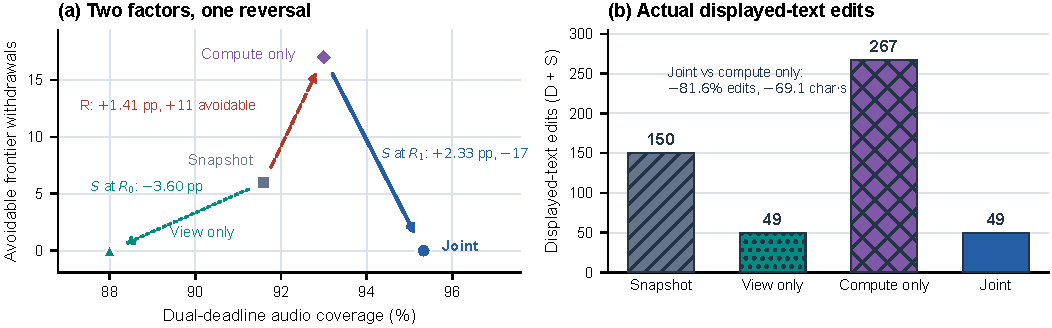
\includegraphics[width=\textwidth]{figures/core_interaction.pdf}
\caption{Joint retention preserves timely, supported progress (714.110
audio-s per arm, three eight-speaker cohorts, primary Qwen, 2-s
feedback, staggered; the four points are discrete policies, not a
measured continuum). (a) Arrows apply one factor: computation retention
alone (dashed) adds 1.41 points and 11 avoidable withdrawals, view
retention alone (dotted) removes six and gives up 3.60 points, both
(solid) gain 2.33 points and remove all 17. (b) Deletions/substitutions
under the primary minimum-distance alignment; final texts are identical
per source.}
\label{fig:main_evidence}
\end{figure*}

Complete dependency paths place each withdrawal at the application that
causes it: snapshot/recompute's 12 split six and six; computation-only's
17 are all avoidable, or 4.6 per 100 offered frontiers; and joint
retention preserves all 18
compatible-ahead opportunities it meets.

A separate 16-session workload makes that distinction visible when
first-delivery credit ranks the policies oppositely: in its third repeat
computation-only credits 201.960~s against 194.735~s, because two 2-s
intervals are withdrawn after credit is assigned. At eight staggered
sessions all arms pass whole-run $D_2/C_8$, yet computation-only still
loses timely supported coverage in 1/2/1 windows and joint retention in
none.

Text revision is another distinct outcome. On actual Consumer strings,
a minimum-distance Unicode alignment gives 267 deletions/substitutions
for computation-only and 49 for joint retention, with modified-identity
lifetimes of 203.297 versus 134.207~character-s, and an alternative
optimal alignment preserves the direction. Joint retention also retires
569 LCP-suffix characters. Final actual text hashes agree per source
across arms, and all five executed arms retain identical complete
selected frontier, result, state, and text histories within each
source/block.

\subsection{What does each switch contribute on the native path?}

\begin{figure*}[t]
\centering
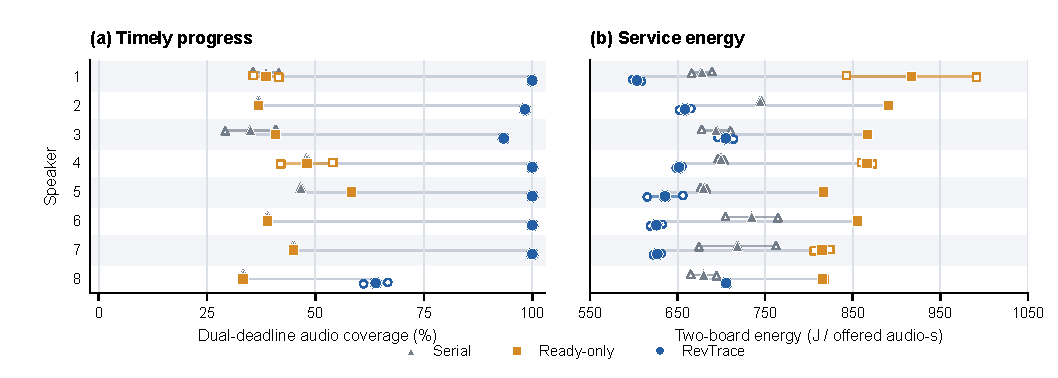
\includegraphics[width=\textwidth]{figures/native_comparison.pdf}
\caption{Timely progress and service energy on the eight-speaker native
workload. The three policies all retain whole supported views; they differ
in whether calls are serial, reusable only after completion, or retained
in flight. These are the same trials as Table~\ref{tab:native_confirmation_v16}:
two fresh-process repeats per speaker and policy from the 80-trial
factorial campaign. Filled markers pool the two repeats; open markers and
short ranges show the individual observations. Speakers use the same
order in both panels. (a) Audio meeting both the 2-s display and 8-s
certification deadlines. (b) Both-board energy from service origin to
confirmed physical model drain, divided by offered audio duration.}
\label{fig:native_comparison}
\end{figure*}
The native comparison isolates a call whose input becomes confirmed while
it is still running. \emph{Fullcall} ($R_1S_1$) keeps that original
complete call; \emph{Ready-only} ($R_0S_1$) can reuse a received,
validated result at the confirmation boundary, but fences an unresolved
call and reissues the work. Both share complete-input checks, original
C/U selection, whole-view support, two workers, ahead limits, and a
canonical-first round-robin dispatcher. The campaign runs each switch in
both positions, plus a policy that issues nothing before confirmation,
on the same eight speakers and 282 offered frontiers.

In-flight retention earns \NativeFullCreditPct\% of the 137.864~offered
audio-s per policy, against \NativeReadyCreditPct\% for completed-result
reuse and \NativeConsCreditPct\% for serial execution: 51.83 points over
reuse and 54.01 over no speculation. All eight sources move the same way
at both view settings, and the paired diagnostic is $2/256=0.0078$ for
each, the smallest value attainable with eight sources.

Fencing is not what produces the gap, and reuse is exercised. At this
500-ms cadence a fenced call's reissued work can display only after
confirmation plus a full inference, so a completed result is rarely
ready in time; one was, on S0907, and was reused. Its 3.000-audio-s
margin over no speculation therefore prices readiness rather than
fencing, at 65\% more worker time.

The two switches act on different quantities. At fixed view retention
the call is worth 71.460~s; at fixed call retention the view is worth
$-1.000$~s; the interaction is $-1.500$~s, so this runtime does not
establish a positive first-credit synergy. What it establishes is the
classification. Replacing the view clears all 10 compatible ahead views
the retaining call meets, on three of the eight sources, and all 13 when
the call is fenced; keeping the view clears none in either position.
Joint retention still withdraws twice, on S0902 in both repeats, where a
new canonical boundary refutes the old prediction: it withholds
incompatible views rather than all withdrawals.

Retained credit hides loss here as well. In-flight retention with the
replacing view earns 130.960~s, 1.000~s more than joint retention, while
removing 5.000~s of supported displayed audio in ten windows of
32--134~ms (median 63) and leaving 0.379~audio-s$\times$wall-s of
avoidable absence; joint retention's only removals are the two refuted
views, and its avoidable absence is zero. All 39 loss windows in the
campaign return within the same root, none censored or truncated. Which
arm leads on first credit is thus workload-dependent, as in the core
study; the class each switch removes is not. Avoidable withdrawal is not
rarer here, only shorter: it occurs at 3.5 per 100 offered frontiers
against 4.6 in the core study, and its length is set by when the next
compatible application arrives.

Worker occupation is \NativeFullWorkerSeconds~s against
\NativeReadyWorkerSeconds~s, and both-board energy is 89.848 against
117.826~kJ: reductions of 31.8\% and 23.7\% against reuse. Against
serial execution the trade partially reverses, because retention spends
12.6\% more worker time (222.523 versus 197.573~s) to serve the same
stream earlier while using 7.4\% less two-board energy (89.848 versus
96.985~kJ). The two comparisons answer different questions and are not
one dominance claim. Relative to Ready-only, every source improves on
credit and energy after pooling its two repeats
(Fig.~\ref{fig:native_comparison}).

\begin{table}[t]
\centering
\caption{Native retention policies: eight speakers, two fresh repeats,
137.864~audio-s and 282 offered frontiers per policy. R0 uses received
complete results only; R1 also keeps a call whose input is confirmed
while it runs. S0 replaces the whole view at a canonical application;
S1 keeps it when the support check passes. Conservative issues no work
ahead of confirmation. Work is occupied-worker wall time; energy covers
both boards to confirmed physical model drain.}
\label{tab:native_confirmation_v16}
\scriptsize\setlength{\tabcolsep}{2.4pt}
\begin{tabular}{@{}lrrrrrr@{}}
\toprule
Policy & $A_{2,8}$ (s) & Cov. & Pass & Av./Nec. & Work (s) & kJ\\
\midrule
Conservative & 55.500 & 40.26\% & 0/16 & 0/0 & 197.573 & 96.985\\
$R_0S_0$ & 58.000 & 42.07\% & 0/16 & 13/6 & 326.546 & 118.632\\
$R_0S_1$ & 58.500 & 42.43\% & 0/16 & 0/6 & 326.232 & 117.826\\
$R_1S_0$ & 130.960 & 94.99\% & 10/16 & 10/2 & 222.646 & 92.814\\
$R_1S_1$ & 129.960 & 94.27\% & 10/16 & 0/2 & 222.523 & 89.848\\
\bottomrule
\end{tabular}
\end{table}


Credit and whole-run passing retain different resolution. S0901 misses
$D_2$ only at EOS; S0902 misses twice at EOS and twice mid-utterance;
S0915 supplies 11 of the 13 non-EOS misses, which is why joint retention
passes 10/16 runs against 0/16 for Ready-only. No arm misses $C_8$ in
these 80 runs, so every miss in Table~\ref{tab:native_confirmation_v16}
is a display miss; the shorter bank never makes the deadline bind.



An earlier two-policy campaign on the same speakers reproduced aggregate
credit within 0.500~audio-s (129.460 against 129.960) and the same 10/16
passes, with 20 against 19 $D_2$ misses.

\subsection{Where the certification deadline binds}

Longer inputs expose it. On a second natural corpus---the lexicon first
four of 29 qualifying MAGICDATA Mandarin speakers~\cite{magicdata68},
one complete 14.396--15.232~s utterance each, frozen before any
transcript is read, three policies twice per speaker over 119.844~audio-s
and 244 frontiers---serial execution misses $C_8$ 27 times at up to
11.508~s, and both retaining arms miss it zero times, at 6.962 and
6.473~s. All 27 are $D_2$ misses as well, so the gain is a deadline met
rather than new $A_{2,8}$ intervals.

The same corpus separates the two retentions where credit cannot: both
earn 65.29275~audio-s against 38.000 for serial execution, identical to
the last digit, yet computation-only clears five compatible ahead views
that joint retention keeps and removes 2.500~audio-s of supported
display. AISHELL separated the arms by 1~s of credit; here only
availability tells them apart.

Serving earlier here costs 35.3\% more worker time and 13.3\% more
energy than serial execution, and all 24 runs reproduce the original
reference state, correction, and returned IDs.

\subsection{Which evidence permits retained work to be used?}
Among 92 model-active input confirmations in an earlier four-source
bank, 20 calls' tentative successor states differ from their final
original C/U results: inputs become valid while predictions are revised,
and retaining the computation leaves selection to the original program.

The six-policy, two-speaker pilot measures the corresponding execution
opportunity. Its 24 cells bind 1,200 actual Consumer rows to original
facts and received ASR/full-result paths. Fullcall has 56 model-active
handovers, each spanning the actual parent-receipt-to-install interval
and later selected for use. Ready-only has zero complete-result hits in
this pilot and 56 same-input reissues. Nine times, a complete result
finished only after its frontier had been fenced and was refused;
retaining the call would have used it.
Over 33.11625~offered audio-s per policy, Fullcall earns 32.340125~s
versus 12.5~s for Ready-only, with 51.765 versus 82.145~worker-s.

The \emph{dependency-versioned} policy realizes the same 56 handovers
and the same credit as Fullcall. Shadow predicates evaluated on the
five speculative policies' recorded schedules agree at all 290 sampled
job/install boundaries: 278 current-input matches and 12 refutations.
A state-bound version representation can therefore implement the same
input witness. The birth-root-fenced auxiliary
records no promotion and earns 12.000~s, equal to Conservative in this
pilot, because it revokes a call when its birth root changes even if the
complete input is later confirmed.

\emph{Unconditional in-flight retention} (UIR) refuses the same two
known-wrong complete returns but suppresses early skip hints; Fullcall
exits before learned correction there and earns 1.5~s more, both on
S0901. The trace thus separates refusal from resource outcome.

\subsection{Can agreement-based publication compose with retention?}
We adapt LocalAgreement-2's consecutive-new-input prefix
decision~\cite{machacek2023whisperstreaming} above the actual recorded
pilot candidates. Original ASR already uses AlignAtt~\cite{papi2023alignatt};
C/U, retained computation, and selected $G$ stay fixed. The adapter
compares Unicode code points and maps a stable prefix to an actually
delivered whole view with a supported complete path. Its audio frontier
comes from that view. Same-frontier ASR/full-C publications supply one
new-input update, and EOS release waits for actual final C/U delivery.

Here canonical-only gates first publication of provisional results;
the core $S$ factor instead governs retention at canonical application.
On Fullcall's four fixed schedules, actual-SUP credit is 32.340125~s,
canonical-only 30.840125~s, and LA2-CP 31.340125~s, over 33.11625~s.
LA2-CP removes all four modified characters for 1~audio-s of credit,
and its within-D2 coverage integral falls from 32.740 to
24.403~audio-s$\times$wall-s under the same right-censored allowance; a
0.5-s fixed-lag control yields 26.840~s, nine modified characters, and
three frontier retreats. The publication choice therefore trades
delivery timing against revision and coverage duration. The observer evaluates four rules on 24 recorded schedules and passes 28
unit tests.

\subsection{Which workloads provide useful retention opportunities?}
At two synchronous native sessions, Fullcall earns 11.5~s versus
Conservative's 10.5~s over 33.11625~s; at four, it earns 9~s versus
10~s over 66.91~s. All eight runs fail whole-run D2. Conservative can
occupy both GPUs with independent canonical chains, and the shared
canonical-first dispatcher issues no conditional work in the four-session
Fullcall cells. Available resources and competing canonical demand
determine whether that execution supplies in-flight work to retain.

Credit reverses under fresh timing: a staggered cohort-A run gives joint
retention 226.320~s against 230.565~s, and pooled synchronous arrivals
$-0.790$~s with $I=+2.565$~s, while it still preserves five and three
compatible-ahead opportunities. Credit tracks timing; which class a
factor removes does not.

\subsection{Do the checks preserve the intended authority?}
The native reference and Consumer checks bind complete inputs, original
C/U, and received whole-view paths. The CPU protocol suite passes
225 unit tests. A bounded hand-written model passes 35 named checks, including
its 27 original controls, over dispatch, ASR, original-C/U, durable-install,
and Consumer actions. Actual process-failure trials separately retain
two matching acquired complete results through producer exit and refuse
two mismatches against their actual parents. Together these checks
exercise the declared trust and ownership boundaries; the original
program, complete-state adapter, and synchronized storage remain their
trusted interfaces.

\subsection{What does the complete synchronous path cost?}
Eight instrumented native trials measure the complete fact and
Consumer paths. The observed mean commit takes 20.35--27.25~ms, or
4.1--5.5\% of the 500-ms input interval; 15.78--22.18~ms lies inside
its synchronous filesystem call, and a whole-view Consumer application
takes 18.58--23.91~ms. These operations bind the complete original
result and parent, persist the selected transition, and apply it to the
actual view that the end-to-end comparisons above measure.

\section{Related Work}\label{sec:related}
\paragraph{Incremental information and dependency reuse}
Incremental dialogue processing represents dependencies between units
and propagates revocation~\cite{schlangen2011incremental}; its commitment
promises that a unit will not be revoked. RevTrace's certification
records selection by the original feedback program, whose later
corrections can still revise the transcript. Adapton validates recorded
dependencies, Nominal Adapton recovers reusable computation by name and
argument, and Differential Dataflow maintains incremental results across
versions~\cite{hammer2014adapton,hammer2015names,mcsherry2013differential}.
These are foundations for the complete-input witness. Our author-built
version-DAG control uses the same complete-input, selection, and
view-support checks as RevTrace and adds revocation after an ancestor
is refuted. Both retain the observed compatible native handovers; the
convergence case in Section~\ref{subsec:ancestor_outlives} explains
where that additional revocation rule can discard a future call before
its own input resolves.

\paragraph{Revisable speech services and speculation}
Whisper-Streaming makes an offline Whisper
recognizer~\cite{radford2023whisper} incremental through
LocalAgreement~\cite{machacek2023whisperstreaming}. StreamCorrect adds
learned correction and feeds the selected text back into later
recognition~\cite{vu2026streamcorrect}. RevTrace retains that original
ASR/Correct/Update program while coordinating asynchronous full calls
and the Consumer's whole view. LocalAgreement-2/3 controls and
prefix-to-prefix commit rules for simultaneous
translation~\cite{ma2019stacl} address the complementary publication
decision. Our fixed-schedule LA2-CP control applies a common-prefix rule
above the native AlignAtt-based kernel~\cite{papi2023alignatt}. It
measures the display tradeoff on recorded candidate schedules with
original correction and feedback unchanged.

SSBD reuses the previous translation as a draft, verifies it under
updated input, and masks displayed suffixes; PredGen generates candidate
replies while input is evolving; RelayS2S commits a verified fast-path
prefix that constrains slow-path generation
\cite{zeng2026ssbd,li2025predgen,mai2026relays2s}. RevTrace keeps that
rule: a confirmed input permits the call's full original result, while
its predicted successor stays subject to original correction. ASR
alignment-drift work shows the
importance of audio-position state~\cite{wang2026alignmentdrift}; that
state is part of our complete-input contract.

\paragraph{Inference reuse and verification}
Orca schedules transformer iterations, PagedAttention and RadixAttention
share KV blocks and token prefixes, and speculative decoding with
tree-based verification accepts draft
tokens~\cite{yu2022orca,kwon2023pagedattention,zheng2024sglang,leviathan2023speculative,miao2024specinfer}.
SGLang also speculates across program primitives by retaining generation
beyond a stop condition and matching it to later operations. RevTrace coordinates
complete frozen feedback calls and binds each retained use to the actual
selected parent. The Consumer then checks the support of its current
whole view. Backend reuse and faster token execution can compose with
this service protocol.

\paragraph{Execution authority and recovery}
Retire separates request-owned resources from execution-version
publication authority and certifies state inheritance under a reuse
contract~\cite{zhang2026retire}. RevTrace derives call and view actions
from selected neural feedback: a view may require withdrawal while a
future input remains unresolved, and an input match leaves original
correction responsible for selecting the successor. We implement
task-level version-DAG and birth-root controls around this same feedback
program.

Optimistic concurrency control validates work before commit;
multiversion control and snapshot isolation supply distinct read
guarantees~\cite{kung1981occ,bernstein1983mvcc,berenson1995isolation}.
Write-ahead logging, distributed snapshots, and lineage restore a
prefix after failure~\cite{mohan1992aries,chandy1985snapshots,zaharia2013dstreams,carbone2017flinkstate}.
RevTrace applies these ordering principles to selected original facts:
it replays the verified prefix, keeps received-result ownership
independent of producer lifetime, and ends physical ownership at
terminal drain rather than lease expiry~\cite{gray1989leases}.

\section{Discussion}\label{sec:discussion}
The results identify two service objectives that require coordination:
making original computation timely and keeping its supported progress
available. First-delivery credit captures the former event; whole-view
support captures the latter state. Their ranking can differ, as the
continuity experiment shows. A service contract therefore needs both a
deadline and a rule for what remains available after feedback changes.

The native comparison isolates a second choice within the same safety
contract: which issued work remains available for reuse. Ready-only and
Fullcall share original selection and view-support checks, but only the
latter preserves a call while its input is being resolved. Input-bound
versions can supply the same eligibility evidence. This gives builders
freedom in representing dependencies while retaining the separate
checks at execution, selection, and application.

\paragraph{What an implementation must preserve}
Three obligations survive any encoding. First, input eligibility:
a representation supports safe in-flight retention only if it can witness
the complete input of the call at the installed parent; a coarse birth
version cannot. Second, original selection: retaining executed work never
endorses its prediction, and the original Correct/Update and the durable
selection boundary stay unchanged. Third, view support: protecting
computation does not protect delivery, so the Consumer validates the
whole view at each actual application. The contract is informational, not
representational: the measured version-DAG policy matches Fullcall's
eligible handovers.

\paragraph{Operating scope}
The measured gains separate a correctness contract from the scheduling
conditions that make reuse profitable: witnesses govern the contract,
while available execution overlap and Consumer timing govern the
profit. Local agreement reduces revisions by waiting for more
evidence; independent canonical chains can consume the slots needed for
conditional execution~\cite{welsh2001seda}. The selected-fact
argument establishes allowed transitions under the execution contract,
while controlled fault injections exercise its lifecycle boundaries.

Adapting this protocol requires a closed, serializably comparable call
boundary: all state read by the original inference and feedback update,
its complete result and selected transition, and the published
dependencies of the Consumer's current view. These interfaces make
eligibility and continued support checkable at the point where retained
work is used. Numerical cross-call state, such as a reused KV cache,
would need an approximate or prefix-matched witness before the same
checks apply.

\section{Conclusion}\label{sec:conclusion}
RevTrace preserves useful progress through trusted feedback revisions by
coordinating original full calls, selected results, and whole consumer
views. The factorial comparison shows why: retaining computation alone
can increase avoidable withdrawals, while view retention alone leaves
timely computation unrecovered. Native full-program comparisons show the
value of preserving work before it is ready to cache: in-flight
retention delivers \NativeFullCreditPct\% dual-deadline coverage against
\NativeReadyCreditPct\% for completed-result reuse and
\NativeConsCreditPct\% when nothing is issued ahead, and on longer
natural utterances it takes certification misses from 27 to zero.
Discarding the view erases every supported view retained calls meet,
buying 1.000~audio-s on the shorter bank and nothing once credit is
equal. The joint protocol resolves each call's own input, retains
original selection authority, and reconciles the actual whole view when
a revision arrives; it composes with agreement-based publication where
stability outweighs an audio-second, and yields where canonical demand
saturates the hardware.

\section*{AI Tool Usage}
ChatGPT/Codex assisted literature discovery, drafting, revision
including the refinement exposition, runtime extensions, experiment
orchestration, and analysis code. The authors retain full responsibility.
\clearpage
\bibliographystyle{IEEEtran}
\bibliography{refs,formal_refs,coordination_refs}
\end{document}
